\documentclass[10pt, a4paper]{aqademic}

\usepackage[spanish]{babel}
	\selectlanguage{spanish}

% Document packages

\usepackage{amsmath}
\usepackage{amsfonts}
\usepackage[type=CC, modifier=by-nc-sa, version=4.0]{doclicense}
\usepackage{tikz}
	\usetikzlibrary{arrows,automata}
\usepackage{tikz-qtree}
\usepackage{graphicx}
	\graphicspath{{img/}}

% Document settings

\author{Atanasio José Rubio Gil}
\title{Modelos de computación}

\AqSetChapter{Práctica}

% Document composition

\begin{document}

\AqMaketitle[%
	cover    = logo-ugr.png,
	org      = Grado en Ingeniería Informática,
	subtitle = Prácticas,
	url      = https://github.com/Groctel/ugr-informatica
]

\begin{titlepage}

\newgeometry{%
	left=5cm,
	right=5cm
}

\thispagestyle{empty}

\topskip0pt
\vspace*{\fill}

\begin{center}
	\textbf{\Huge{¡Gracias por apostar por el conocimiento libre!}}
\end{center}

\vspace{1cm}

Estos apuntes están compartidos libremente para que puedas estudiar de forma gratuita y sin bloques de publicidad molesta en tus páginas.
Su publicación y uso son un paso adelante en la idea de que el conocimiento debería ser compartido de forma libre y gratuita para todos sin ningún tipo de impedimentos o distracciones generadas por muros de pago.

Como autor, no recibo ningún tipo de ingreso por la confección y publicación de este material.
Si quieres colaborar y ayudarme a seguir ofreciéndote facilidades para estudiar, puedes unirte al proyecto a través del enlace de la portada o enviarme una propina mediante el siguiente botón o su enlace:

\vspace{0.5cm}

\begin{center}
	\href{https://ko-fi.com/groctel}{
\includegraphics[scale=0.15]{RecursosTeX/BuyMeACoffee_blue-2x.pdf}}
	\url{https://ko-fi.com/groctel}
\end{center}

\vspace{0.5cm}

Dado que este documento está compartido bajo una licencia \textbf{CC-by-nc-sa}, tienes la libertad de distribuirlo y adaptarlo bajo las siguientes condiciones:

\begin{itemize}
	\item\textbf{BY:} Debes darme crédito de forma adecuada con un enlace a la licencia e indicar si has hecho cambios.
	\item\textbf{NC:} No puedes hacer uso del mismo con propósitos comerciales.
	\item\textbf{SA:} Debes distribuir tus modificaciones bajo la misma licencia que el documento original.
\end{itemize}

Puedes leer la licencia completa pinchando en el enlace de la portada.

\vspace*{\fill}

\end{titlepage}

\tableofcontents

\chapter{}

\section{Enunciado}

Analizar y probar gramáticas libres y dependientes del contexto con jFlap.

\section{Solución}

Vamos a trabajar primero con la siguiente gramática libre del contexto:

\begin{align*}
	G &= (V, T, P, S) : \\
	V &= \{S, A, B\} \\
	T &= \{a, b\} \\
	P &=
		\begin{cases}
		\begin{array}{ll}
			S \rightarrow aB & A \rightarrow bAA \\
			S \rightarrow bA & B \rightarrow b   \\
			A \rightarrow a  & B \rightarrow bS  \\
			A \rightarrow aS & B \rightarrow aBB \\
		\end{array}
 		\end{cases} \\
	S &= S
\end{align*}

La introducimos en jFlap:

\begin{figure}[h!]
\begin{center}
	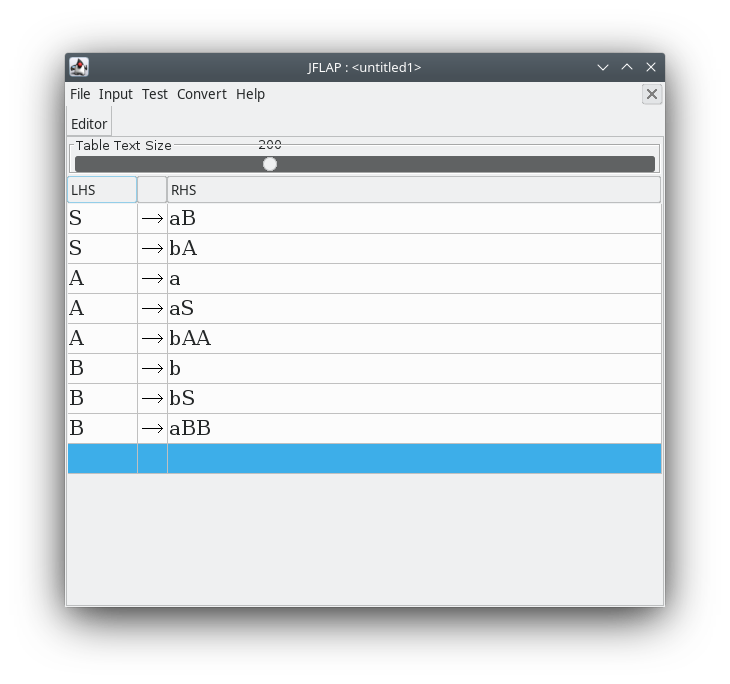
\includegraphics[scale=0.4]{Prácticas/jFlap - Gramática libre del contexto}
\end{center}
\caption{Introducción de la primera gramática en jFlap.}
\end{figure}

\pagebreak

Procedemos a ejecutarla:

\begin{figure}[h!]
\begin{center}
	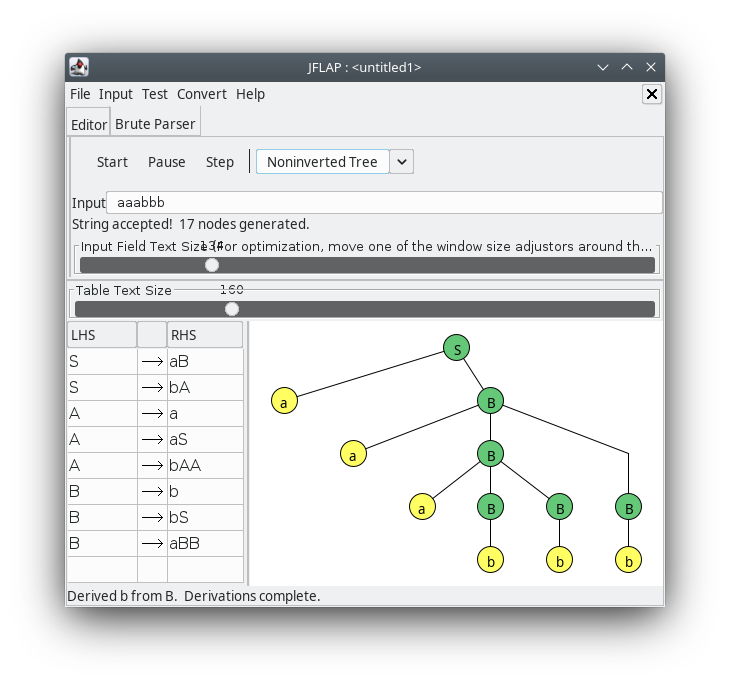
\includegraphics[scale=0.4]{Prácticas/jFlap - Gramática libre del contexto ejecución}
	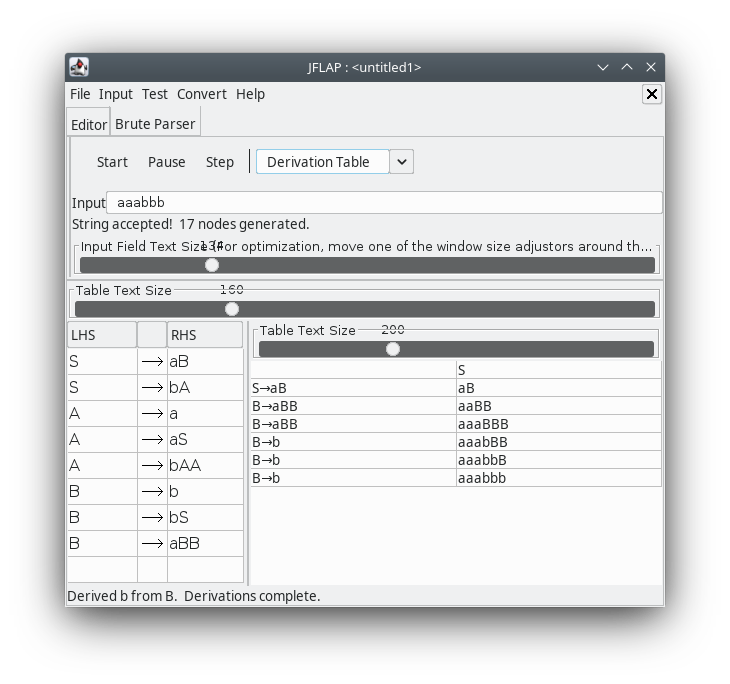
\includegraphics[scale=0.4]{Prácticas/jFlap - Gramática libre del contexto derivación}
\end{center}
\caption{Ejecución y tabla de derivación de la primera gramática en jFlap.}
\end{figure}

Vamos ahora a trabajar con la siguiente gramática dependiente del contexto:

\begin{align*}
	G &= (V, T, P, S) : \\
	V &= \{S, X, Y\} \\
	T &= \{a, b, c\} \\
	P &=
		\begin{cases}
		\begin{array}{ll}
			S \rightarrow abc   & bY \rightarrow Yb  \\
			S \rightarrow aXbc  & aY \rightarrow aaX \\
			Xb \rightarrow bX   & aY\rightarrow aa   \\
			Xc \rightarrow Ybcc &                    \\
		\end{array}
 		\end{cases} \\
	S &= S
\end{align*}

\pagebreak

La introducimos en jFlap:

\begin{figure}[h!]
\begin{center}
	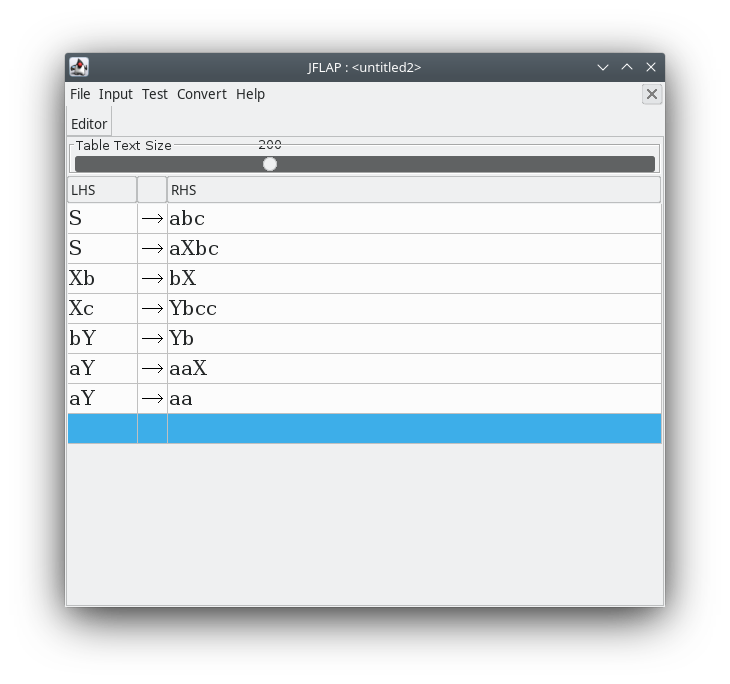
\includegraphics[scale=0.4]{Prácticas/jFlap - Gramática dependiente del contexto}
\end{center}
\caption{Introducción de la segunda gramática en jFlap.}
\end{figure}

Procedemos a ejecutarla:

\begin{figure}[h!]
\begin{center}
	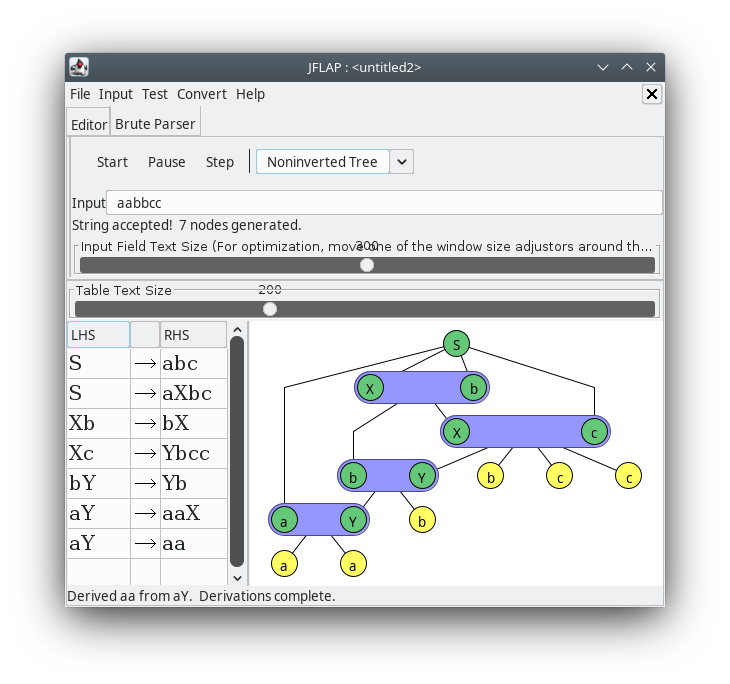
\includegraphics[scale=0.4]{Prácticas/jFlap - Gramática dependiente del contexto ejecución}
	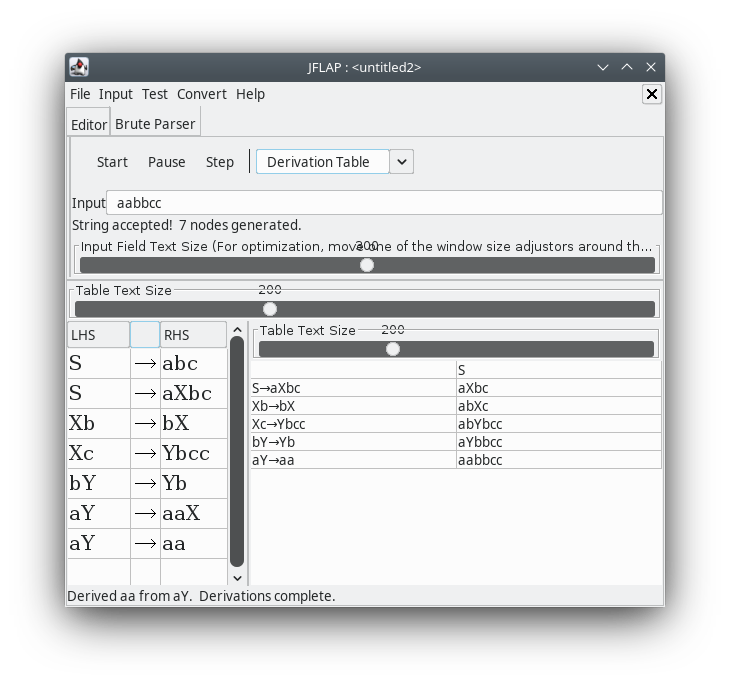
\includegraphics[scale=0.4]{Prácticas/jFlap - Gramática dependiente del contexto derivación}
\end{center}
\caption{Ejecución y tabla de derivación de la segunda gramática en jFlap.}
\end{figure}

\chapter{}

\section{Enunciado}

Usar expresiones regulares y Lex para detectar cadenas dentro de un texto.

\section{Solución}

Trabajamos con el siguiente código de Lex:

\begin{lstlisting}[language=c]
minuscula [a-z]
mayuscula [A-Z]
numero    [0-9]

letra     ({minuscula}|{mayuscula})
normal    ({letra}|{numero})

usuario   (\@{letra}+)
dominio   (\.{letra}+)
byte      ((((""|1)(""|[1-9]))[0-9])|(2[0-4][0-9])|(25[0-5]))

dir_ip    (({byte}\.){3}{byte})
web       ({normal}+{dominio})
correo    (({normal}|"_")+\@{dominio})

%%

{usuario} {printf("Usuario válido: '%s'\n", yytext);}
{dominio} {printf("Dominio válido: '%s'\n", yytext);}
{byte}    {printf("Byte válido:    '%s'\n", yytext);}
{dir_ip}  {printf("Dir_ip válido:  '%s'\n", yytext);}
{web}     {printf("Web válido:     '%s'\n", yytext);}
{correo}  {printf("Correo válido:  '%s'\n", yytext);}
.+

%%

int yywrap ()
{
	return 1;
}

int main ()
{
	yylex();
	return 1;
}
\end{lstlisting}

\pagebreak

Lo compilamos con las siguiente órdenes:

\begin{lstlisting}[language=sh]
lex -o practica2.c practica2.l
gcc practica2.c -o practica2
\end{lstlisting}

Por último, lo ejecutamos y producimos la siguiente salida:

\begin{lstlisting}
@groctel
Usuario válido: '@groctel'

ugr.es
Web válido:     'ugr.es'

143
Byte válido:    '143'

0.0.0.0
Dir_ip válido:  '0.0.0.0'

255.123.12.96
Dir_ip válido:  '255.123.12.96'

.com
Dominio válido: '.com'

deiit@ugr.es
Correo válido:  'deiit@ugr.es'
\end{lstlisting}

\chapter{}

\section{Enunciado}

Implementar un codificador y decodificador de mensajes haciendo uso de máquinas de Mealy.

\section{Solución}

Vamos a crear una máquina de Mealy que codifique un mensaje que trabaje con dos procesos de codificación:
Invertir ceros ($q_0$) y unos o reproducirlos sin inversión ($q_1$).
La máquina empezará codificando en el primer modo y, después de leer un \texttt{1} y codificarlo en el modo actual, cambiará de modo.

\begin{figure}[h!]
\begin{center}
	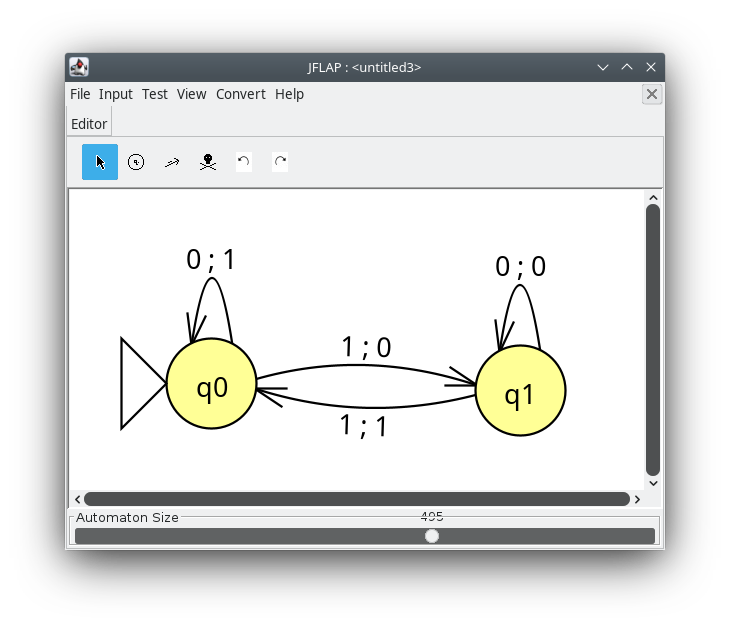
\includegraphics[scale=0.34]{Prácticas/Mealy - Codificador}
	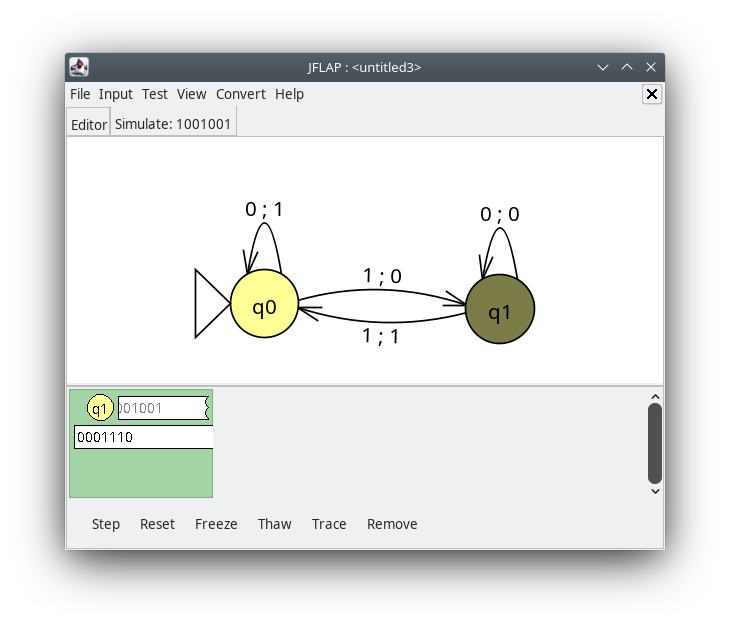
\includegraphics[scale=0.34]{Prácticas/Mealy - Codificador ejecución}
\end{center}
\caption{Máquina de Mealy codificadora.}
\end{figure}

Para crear un decodificador, hacemos lo mismo pero indicando que el cambio de modo se realice después de leer un \texttt{0}.
Lo probamos introduciendo la cadena resultante de la ejecución anterior.

\begin{figure}[h!]
\begin{center}
	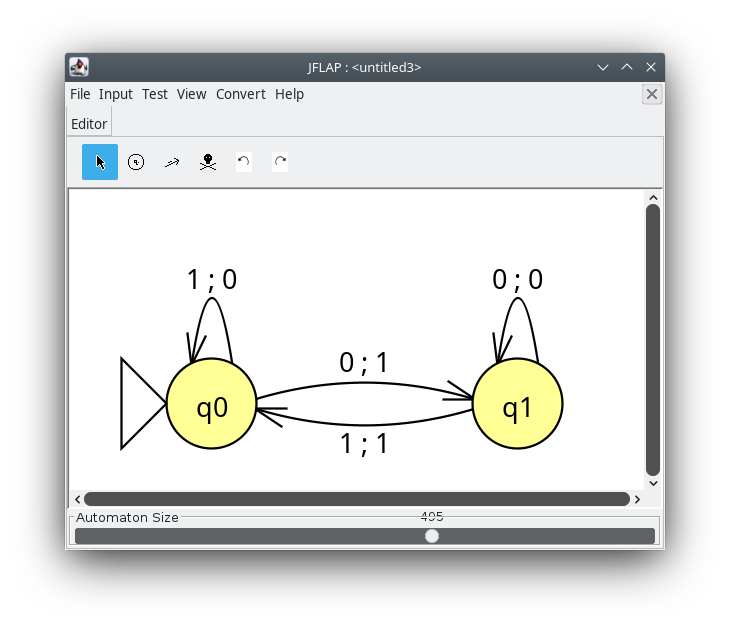
\includegraphics[scale=0.34]{Prácticas/Mealy - Decodificador}
	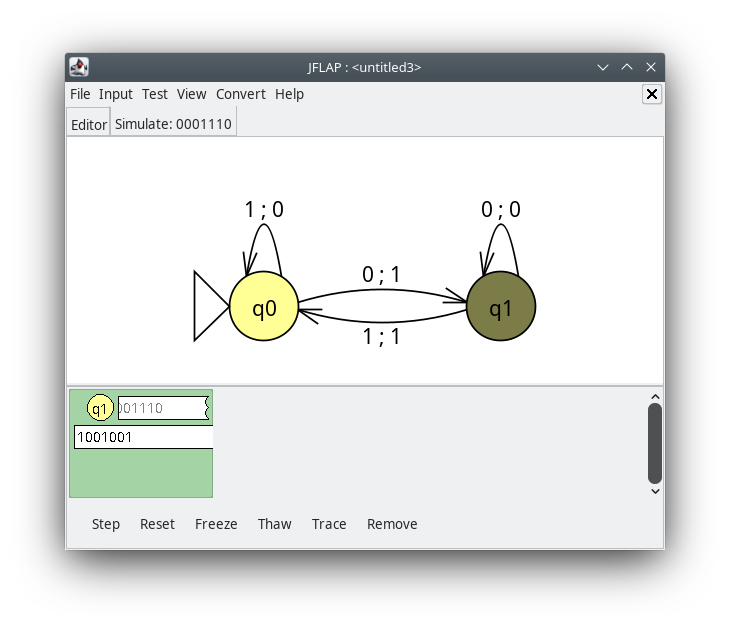
\includegraphics[scale=0.34]{Prácticas/Mealy - Decodificador ejecución}
\end{center}
\caption{Máquina de Mealy decodificadora.}
\end{figure}

\chapter{}

\section{Enunciado}

Dado un autómata con pila configurado para acabar por el criterio de pila vacía, modificarlo para que funcione con el criterio de estados finales.

\section{Solución}

Vamos a generar el autómata mencionado en el enunciado:

\begin{figure}[h!]
\begin{center}
	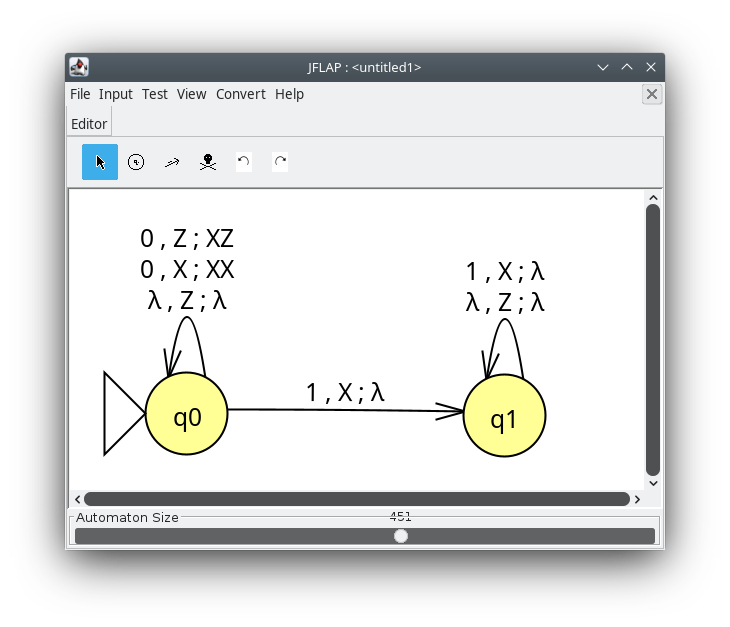
\includegraphics[scale=0.32]{Prácticas/Pila - Pila vacía}
	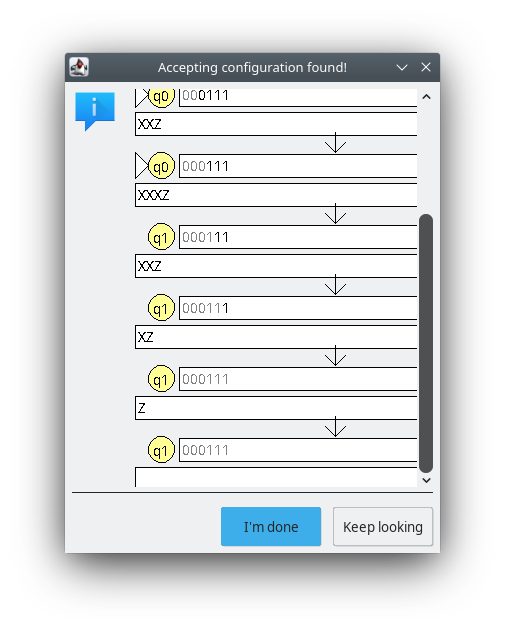
\includegraphics[scale=0.32]{Prácticas/Pila - Pila vacía ejecución}
\end{center}
\caption{Autómata con pila funcionado con el criterio de pila vacía.}
\end{figure}

El problema que tiene este autómata es que no acepta cadenas nulas al usar el criterio de estados finales.
Queremos que este ocmportamiento funcione porque el autómate acepta cadenas con tantos ceros como unos, por lo que la cadena vacía debe ser correcta (ningún cero y ningún uno).
Vamos a modificarlo y comprobar que acepta cadenas vacías:

\begin{figure}[h!]
\begin{center}
	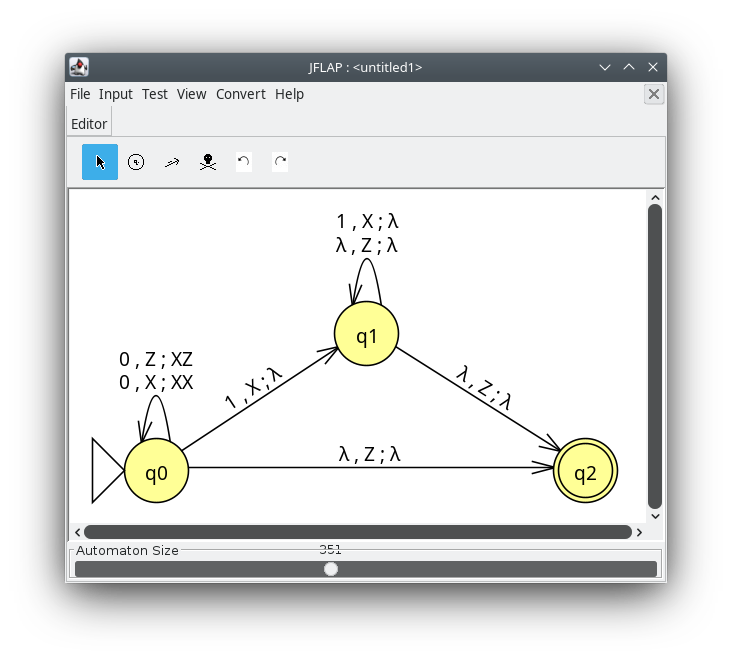
\includegraphics[scale=0.32]{Prácticas/Pila - Estados finales}
	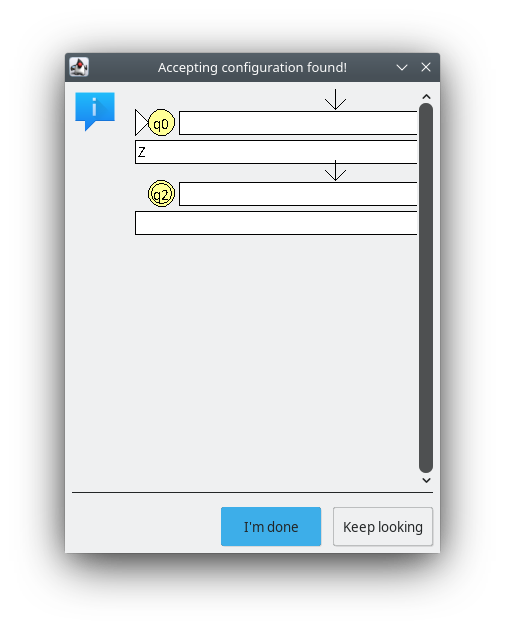
\includegraphics[scale=0.32]{Prácticas/Pila - Estados finales ejecución}
\end{center}
\caption{Autómata con pila funcionado con el criterio de estados finales.}
\end{figure}


\end{document}
